\documentclass[]{beamer}



% Class options include: notes, notesonly, handout, trans,
%                        hidesubsections, shadesubsections,
%                        inrow, blue, red, grey, brown

% Theme for beamer presentation.
\usepackage{beamerthemesplit} 
% Other themes include: beamerthemebars, beamerthemelined, 
%                       beamerthemetree, beamerthemetreebars  
\usepackage{listings}
\usepackage{color}
\usepackage{graphicx}
\definecolor{dkgreen}{rgb}{0,0.6,0}                     %
\definecolor{gray}{rgb}{0.5,0.5,0.5}                    %
\definecolor{mauve}{rgb}{0.88,0.1,0.82}                 %
\definecolor{backcolour}{rgb}{0.95,0.95,0.92}           %
                                                        %
\lstset{frame=tb,                                       %
  language=C,                                           %
  aboveskip=3mm,                                        %
  belowskip=3mm,                                        %
  showstringspaces=false,                               %
  columns=flexible,                                     %
  basicstyle={\small\ttfamily},                         %
  numbers=none,                                         %
  numberstyle=\tiny\color{gray},                        %
  keywordstyle=\color{blue},                            %
  commentstyle=\color{dkgreen},                         %
  stringstyle=\color{mauve},                            %
  breaklines=true,                                      %
  breakatwhitespace=true,                               %
  tabsize=3,                                            %
  numbers=left,                                         %
  basicstyle=\ttfamily\footnotesize,                    %
  backgroundcolor=\color{backcolour},                   %
  numbersep=5pt,                                        %
  basicstyle= \large \ttfamily                          %
}                                                       %


\title{The build-process in C}    % Enter your title between curly braces
\author{Abdelrahman Aboghanima} 
%\institute{CSE department, Minia Engineering Faculty.}      % Enter your institute name between curly braces
\date{\today}                    % Enter the date or \today between curly braces

\begin{document}

% Creates title page of slide show using above information
\begin{frame}
  \titlepage
\end{frame}
\note{Talk for 30 minutes} % Add notes to yourself that will be displayed when
                           % typeset with the notes or notesonly class options

\section[Outline]{}

% Creates table of contents slide incorporating
% all \section and \subsection commands
\begin{frame}
  \tableofcontents
\end{frame}





\section{What is the build process}


\begin{frame}[fragile]
  \frametitle{What is the build process}   % Insert frame title between curly braces
  The process of converting the \item \verb|.c, .h| files, the human readable code, to machine code.
\end{frame}


\section{Preprpcessor}
\begin{frame}[fragile]
  \frametitle{Preprocessor}
  The preprocessor provides the ability for the inclusion of header files, macro expansions, conditional compilation, and line control. 
\end{frame}

\begin{frame}[fragile]
  \frametitle{Example}

 
  \begin{minipage}[t]{0.45\linewidth}
    \lstinputlisting{ex/func1.h}
  \end{minipage}
  \hfill\vrule\hfill
  \begin{minipage}[t]{0.45\linewidth}
    \lstinputlisting{ex/func1.c}
  \end{minipage}

 \begin{lstlisting}
   $ avr-gcc -E -P func1.c  
 \end{lstlisting}
  
\end{frame}
  

\begin{frame}[fragile]
\frametitle{Preprocessor Output} 
\begin{minipage}[t]{0.45\linewidth}
  \lstinputlisting{ex/func1.i}
\end{minipage}


\end{frame}





\note{The end}       % Add notes to yourself that will be displayed when
		     % typeset with the notes or notesonly class options





\section{Compiler}
\begin{frame}[fragile]
  \frametitle{Compiler}
  The process of converting the portable C code into the architecture specific assembly code

  \begin{lstlisting}
    $ gcc -S func1.c
  \end{lstlisting}

  \begin{lstlisting}
    $ avr-gcc -S func1.c
  \end{lstlisting}

  \begin{lstlisting}
    $ arm-none-eabi-gcc -S func1.c
  \end{lstlisting}
  
\end{frame}

\begin{frame}[fragile]

  \newsavebox{\mybox}
  \begin{lrbox}{\mybox}%

    \begin{minipage}[t]{0.33\linewidth}
        % use scale box for later
        \lstinputlisting[basicstyle=\tiny]{ex/func1.x86}
    \end{minipage}
    
    \hfill\vrule\hfill

    \begin{minipage}[t]{0.33\linewidth}
        \lstinputlisting[basicstyle=\tiny]{ex/func1.arm}
      \end{minipage}

    \hfill\vrule\hfill
    
    \begin{minipage}[t]{0.33\linewidth}
        \lstinputlisting[basicstyle=\tiny]{ex/func1.avr}
      \end{minipage}
    \end{lrbox}
  
    \scalebox{0.55}{\usebox{\mybox}}
  \end{frame}




\section{Assembler}
\begin{frame}[fragile]
  \frametitle{Assembler}
  The process of transforming the architecture assembly code to its assocaiated machine code.

  \begin{lstlisting}
    $ gcc -c func1.s -o func1.x68.o
  \end{lstlisting}

  \begin{lstlisting}
    $ avr-gcc -c func1.s -o func1.avr.o
  \end{lstlisting}

 
  \begin{lstlisting}
    $ arm-none-eabi-gcc -c func1.s -o func1.arm.o
  \end{lstlisting}
  
\end{frame}

\begin{frame}
  

  \begin{figure}[!htb]
    \centering
    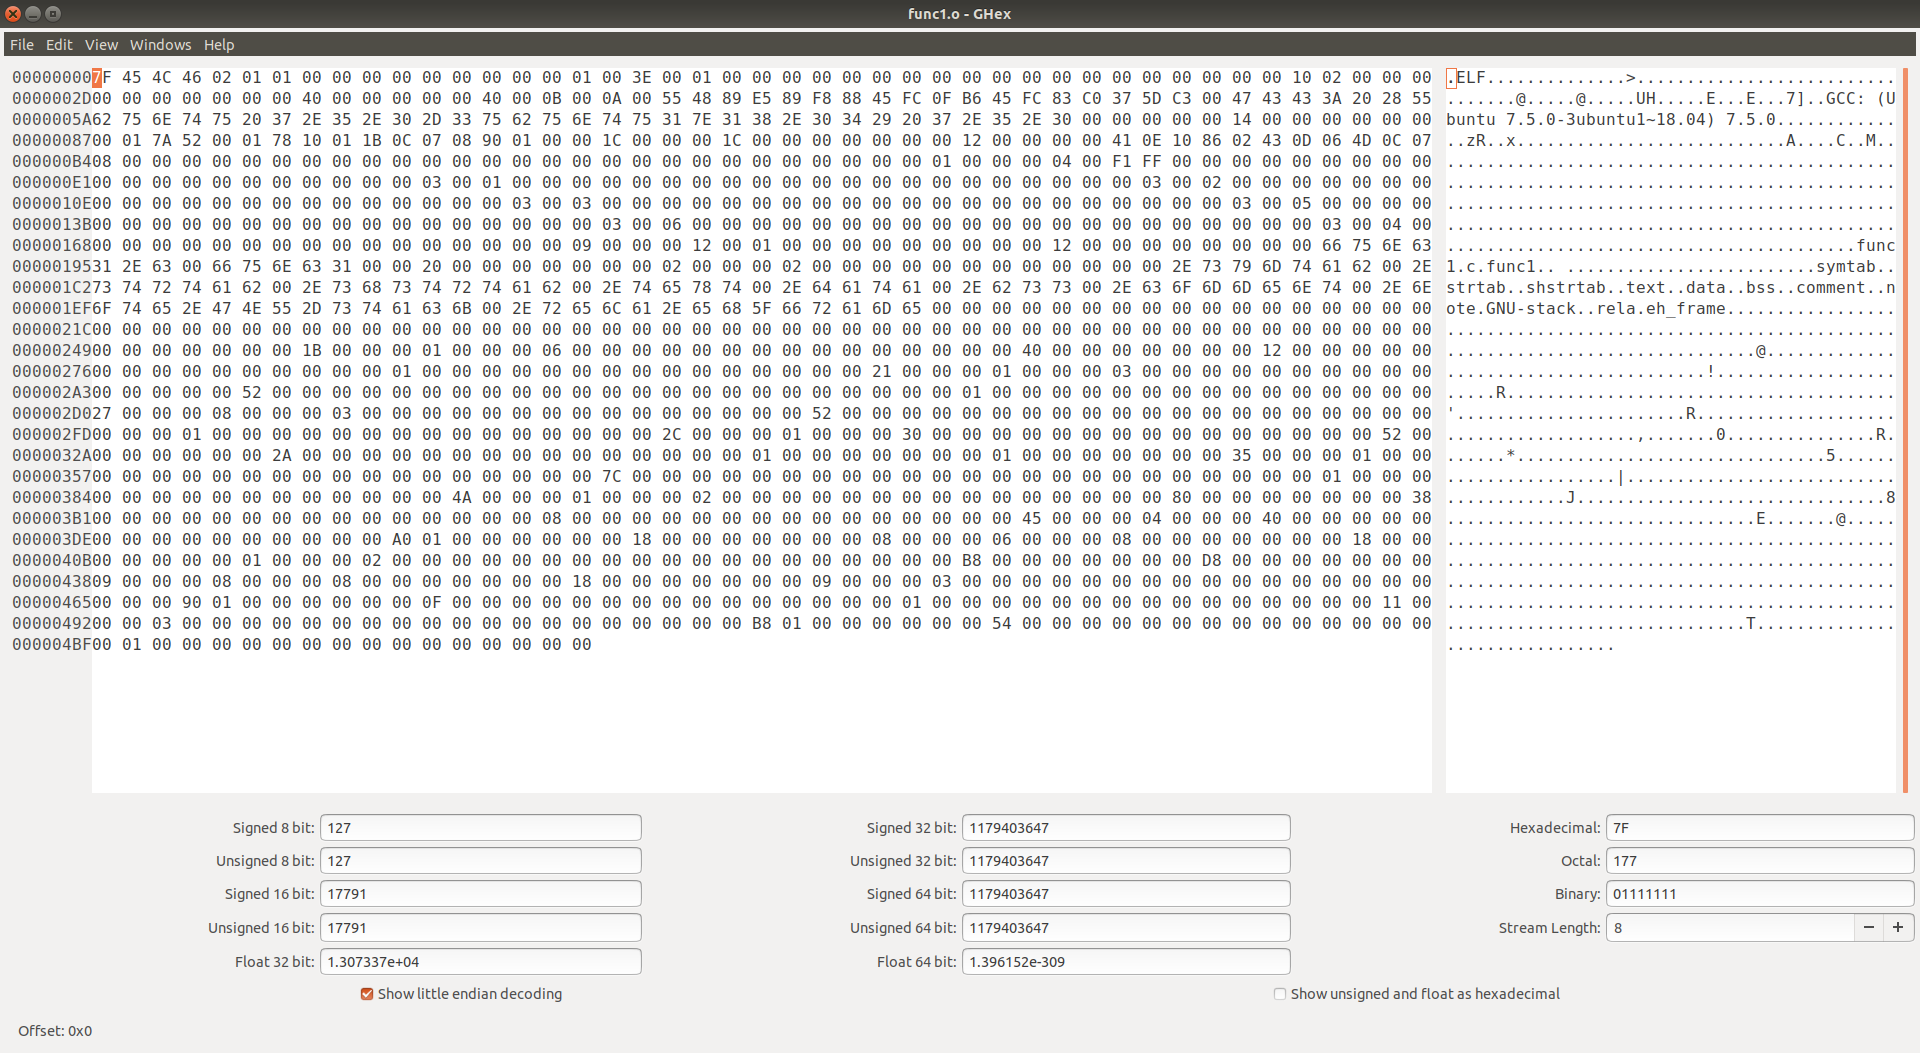
\includegraphics[width=\linewidth]{figures/x86.png}
    \caption{The machine code for x86 architecture.}
    \label{fig:question}
  \end{figure}

\end{frame}


\begin{frame}
  

  \begin{figure}[!htb]
    \centering
    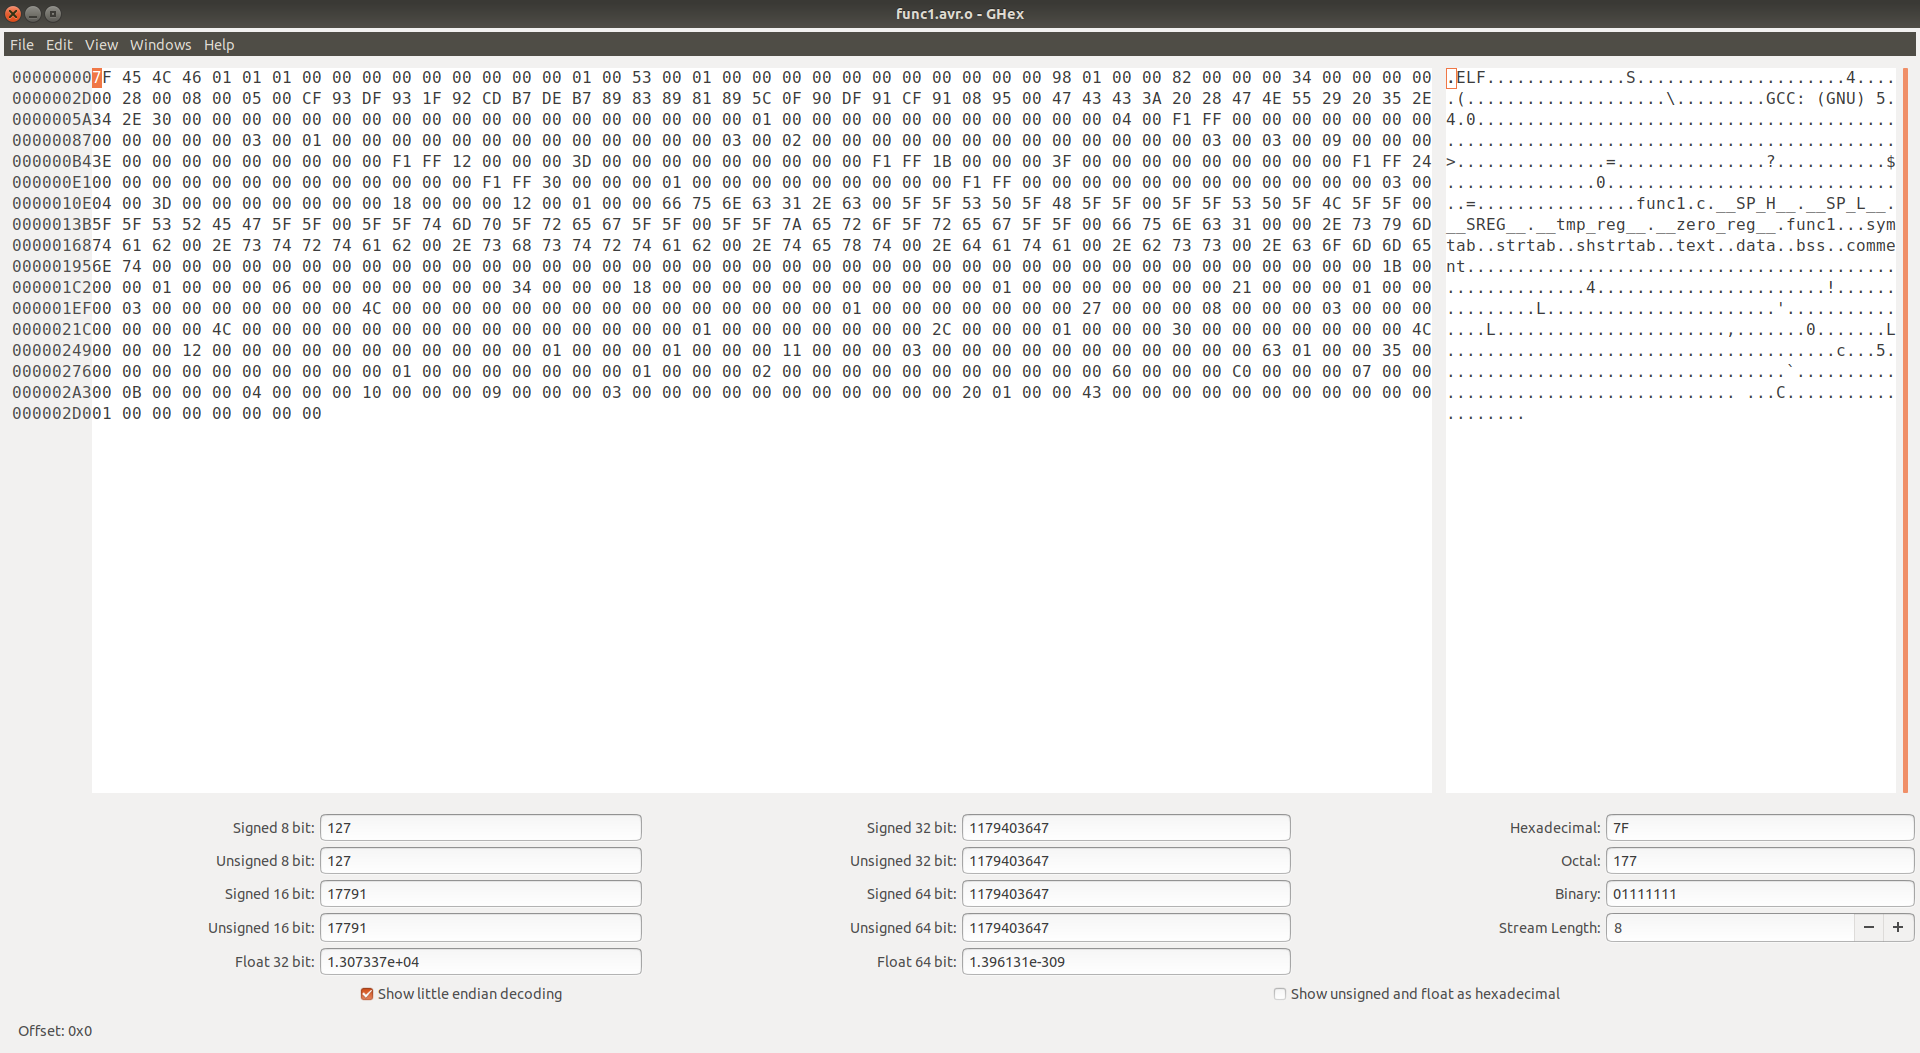
\includegraphics[width=\linewidth]{figures/avr.png}
    \caption{The machine code for avr architecture.}
    \label{fig:question}
  \end{figure}

\end{frame}

\begin{frame}
  

  \begin{figure}[!htb]
    \centering
    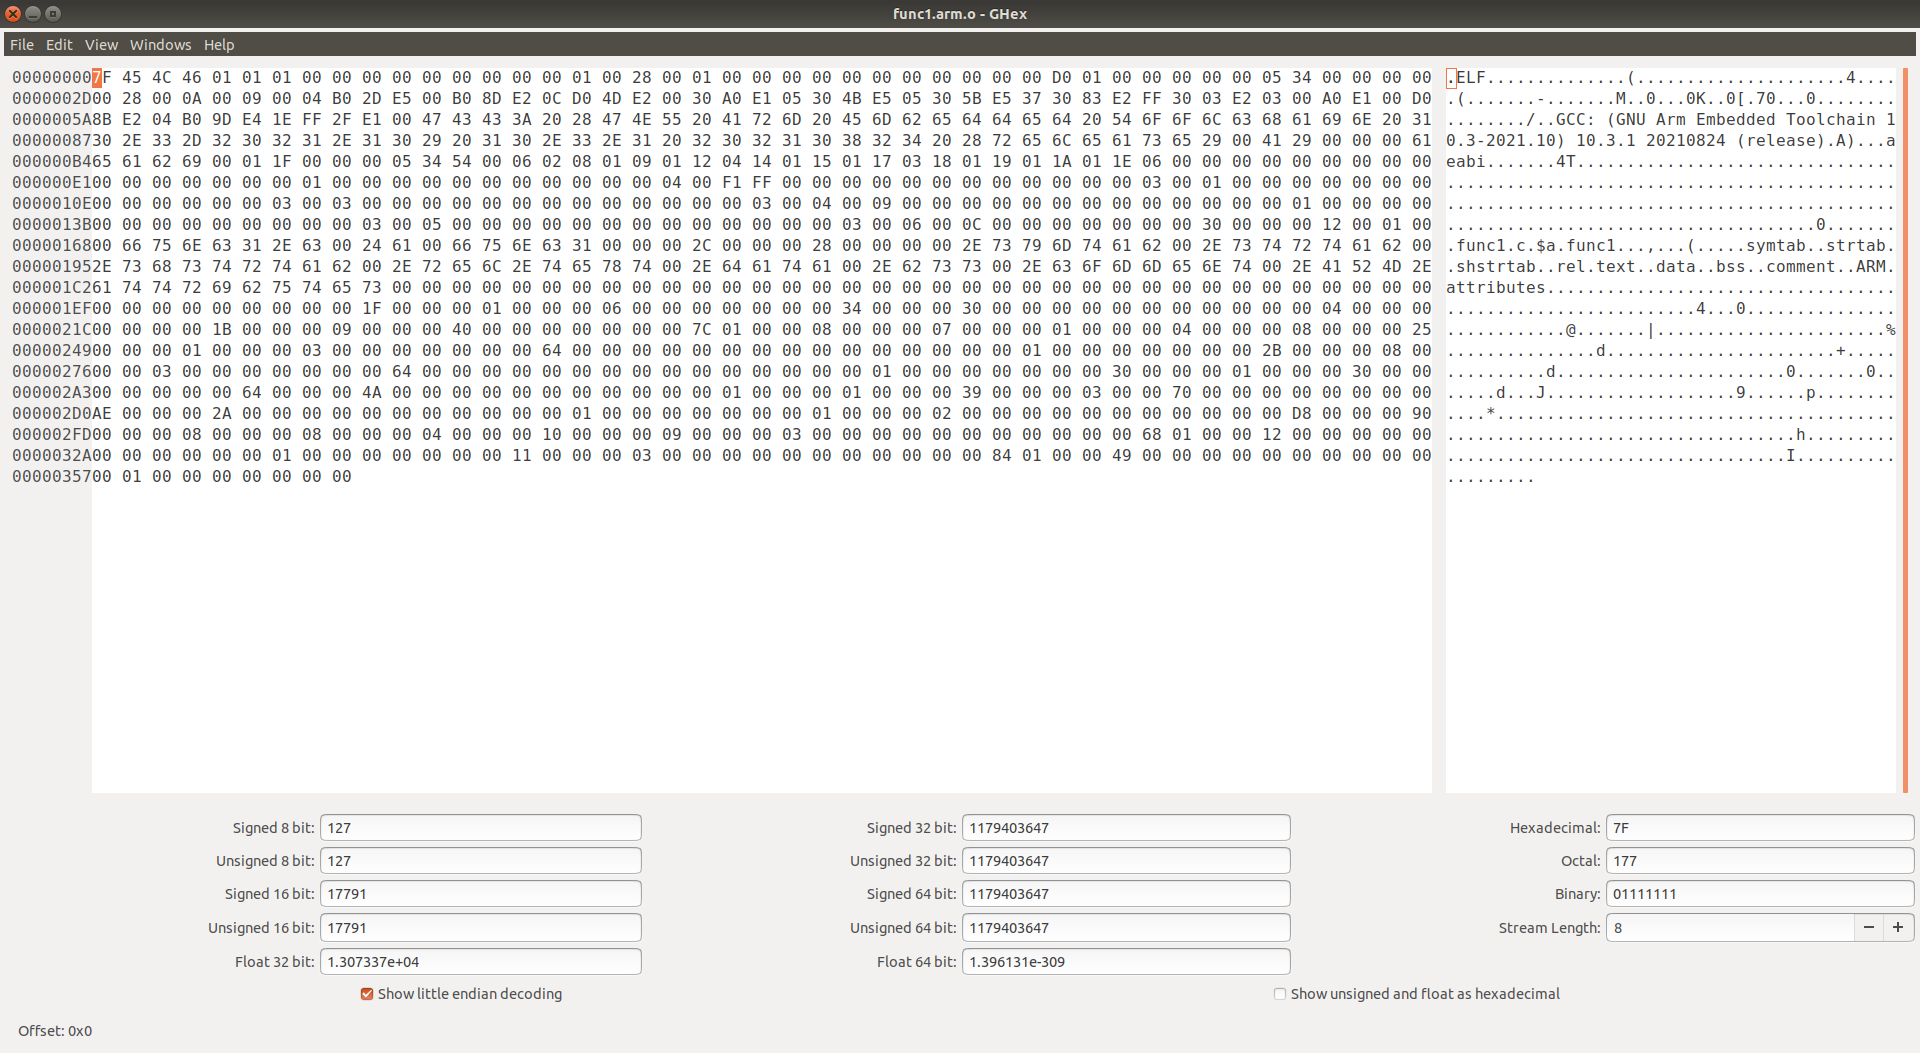
\includegraphics[width=\linewidth]{figures/arm.png}
    \caption{The machine code for arm architecture.}
    \label{fig:question}
  \end{figure}

\end{frame}



\section{Linker}

\begin{frame}
  \frametitle{Linker}
  \begin{Definition}
    \alert{Linker}: is a computer system program that takes one or more object files
    (generated by a compiler or an assembler) and combines them into a single executable file,
    library file, or another "object" file. 
  \end{Definition}
  
\end{frame}

\section{Locator}

\begin{frame}
  \frametitle{Locator}

\end{frame}


\end{document}
